\section{Results}\label{sec:results}

\subsection{Descriptive Duration Profiles}\label{sec:descriptives}
Observed issue-to-closure durations exhibit pronounced right skew (Table~\ref{tab:descriptives} and Fig.~\ref{fig:ecdf}). For single-PR issues (Group A), the median duration is \valmedA{}~days (mean \valmeanA{}~days), with the 90th percentile reaching \valpNinetyA{}~days. In contrast, multi-PR issues (Group B) exhibit substantially higher durations across all percentiles: median \valmedB{}~days (IQR \valqOneB--\valqThreeB~days, mean \valmeanB{}~days), and a 90th percentile extending to \valpNinetyB{}~days.

\begin{figure}[htbp]\centering
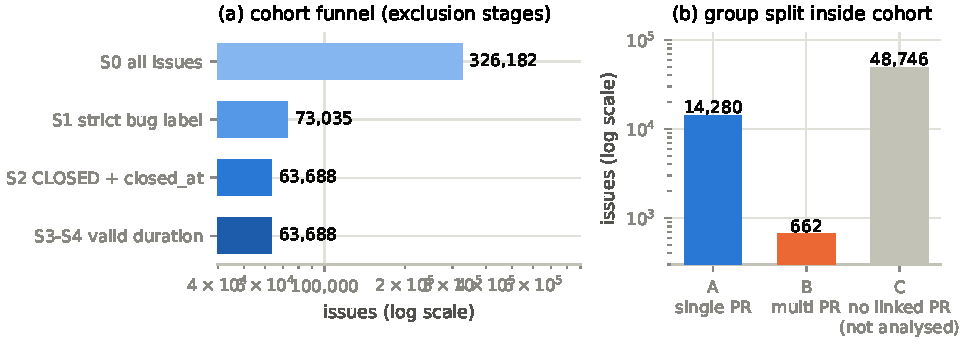
\includegraphics[width=.62\linewidth]{figures/fig1_cohort.pdf}
\caption{Cohort construction pipeline: sequential exclusion stages (panel a) and grouping into Groups A, B, and C (panel b).\label{fig:cohort}}
\end{figure}

\begin{figure}[htbp]\centering
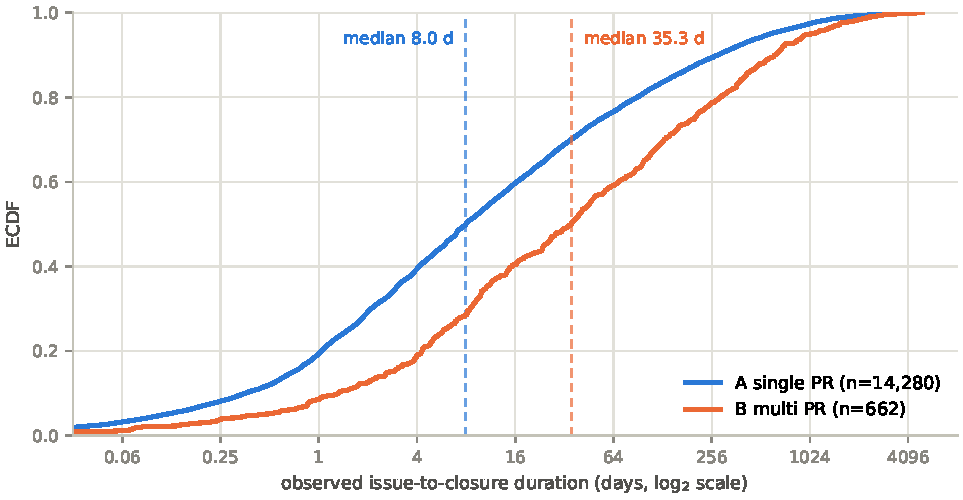
\includegraphics[width=.58\linewidth]{figures/fig2_ecdf.pdf}
\caption{Empirical cumulative distribution function (ECDF) of issue closure duration on a log scale. The multi-PR distribution (Group B) is consistently shifted rightward relative to Group A.\label{fig:ecdf}}
\end{figure}

For context, closed strict bugs without any resolvable linked PR (Group C, 76.5\% of the cohort) have a median duration of 7.8~days, comparable to Group A. Many Group C tickets reflect trivial reports, user configuration issues, or stale tickets closed administratively without code modifications.

\begin{table}[t]
\centering
\caption{Observed issue-to-closure duration (days) by group.\label{tab:descriptives}}
\small \begin{tabular}{@{}llrrrrrrrrr@{}}
\toprule
Group & $n$ & Mean & SD & Q1 & Median & Q3 & P90 & P95 & Max \\\midrule
A (1 PR) & 14,280 & 110.6 & 323.2 & 1.51 & \textbf{8.0} & 54.4 & 280 & 588 & 4,098\\
B ($\geq$2 PRs) & 662 & 219.4 & 485.3 & 5.92 & \textbf{35.3} & 200.6 & 625 & 1,054 & 5,042\\
C (0 PRs, not analysed) & 48,746 & 131.1 & 351.0 & 0.74 & \textbf{7.8} & 71.6 & 363 & 765 & 6,406\\
\bottomrule
\end{tabular}
\end{table}


\subsection{Primary Comparative Analysis: Single-PR vs.\ Multi-PR Bugs}\label{sec:primary}
Table~\ref{tab:main} presents the primary comparative findings: multi-PR issues close systematically later than single-PR issues. The observed median difference is \valmedDiff{}~days, and the Hodges--Lehmann location shift is \valhlShift{}~days, confirming that the entire duration distribution is shifted rightward rather than merely the central tendency.

\begin{table}[t]
\centering
\caption{Primary comparison: single-PR (A) vs.\ multi-PR (B) closed strict bugs. Both confidence intervals use 10{,}000 bootstrap draws (seed 20261120); the project-level one is wider and is the honest reading.\label{tab:main}}
\small \begin{tabular}{@{}ll@{}}
\toprule
Quantity & Value \\\midrule
Samples (Group A / Group B) & 14,280 / 662 issues \\
Median days to closure (A / B) & 8.0 / 35.3 \\
Median difference (B $-$ A) & \textbf{27.3}~days \\
Hodges--Lehmann shift & 9.8~days \\
Mann--Whitney $U$ (two-sided $p$) & 6\,069\,998 ($p=3.31\times 10^{-35}$) \\
Cliff's $\delta$ (magnitude) & 0.284 (small) \\
95\% CI for median difference, resampling issues & [18.3, 35.2] days \\
95\% CI for median difference, resampling projects & [13.9, 51.4] days \\
Within-project sign test & B slower in 88/117 projects ($p=4.28\times 10^{-8}$) \\
Regression $\log(1+\text{days})$, project $\times$ year fixed effects & $\hat\beta=0.905$, CI [0.67, 1.14], $p=3.83\times 10^{-14}$ \\
\bottomrule
\end{tabular}
\end{table}


The Mann--Whitney $U$ test confirms stochastic dominance ($p=\valpPrim$). The Cliff's delta effect size is $\delta = \valcliffsD$ (small-to-medium magnitude), indicating that in roughly 64\% of all random pairings between a Group-B ticket and a Group-A ticket, the multi-PR ticket closed later. 

Crucially, when accounting for project-level clustering, the 10{,}000-draw project-clustered bootstrap 95\% confidence interval spans \valciCluster{}~days. Because this interval comfortably excludes zero, the observed association cannot be dismissed as an artifact of issue clustering across the \valnProjAB{} contributing repositories.

\subsection{Within-Project Consistency}\label{sec:projlevel}
To test whether the observed gap simply reflects multi-PR issues concentrating within chronically slow projects, we examined the \valnProjBoth{} repositories that contribute issues to both Group A and Group B.

\begin{table}[t]
\centering
\caption{Projects with the most Group-B issues (top 15 of 117; the complete list of 117 projects ships with the replication package as \texttt{tables/tab\_projects\_all.tex}).\label{tab:projects-top}}
\small \begin{tabular}{@{}lrrrrr@{}}
\toprule
Project & $n_A$ & $n_B$ & Med.\ A (d) & Med.\ B (d) & Diff (d) \\
rptools/maptool & 626 & 56 & 6.9 & 10.7 & 3.8 \\
openra/openra & 858 & 52 & 20.5 & 117.0 & 96.5 \\
ihhub/fheroes2 & 1,222 & 42 & 8.9 & 116.0 & 107.1 \\
tobymao/18xx & 1,197 & 39 & 1.6 & 7.4 & 5.8 \\
vcmi/vcmi & 798 & 29 & 8.2 & 11.9 & 3.7 \\
draftbot-a-discord-adventure/draftbot & 404 & 24 & 1.8 & 8.8 & 7.1 \\
Crownicles/Crownicles & 404 & 24 & 1.8 & 8.8 & 7.1 \\
revolutionary-games/thrive & 407 & 24 & 23.2 & 99.2 & 76.1 \\
pixijs/pixijs & 235 & 22 & 9.5 & 7.6 & -1.9 \\
gameservermanagers/linuxgsm & 293 & 22 & 30.0 & 24.8 & -5.2 \\
lichess-org/lila & 433 & 21 & 4.8 & 16.8 & 12.0 \\
freeorion/freeorion & 284 & 20 & 6.0 & 11.1 & 5.1 \\
magefree/mage & 206 & 16 & 31.6 & 483.5 & 451.9 \\
CorsixTH/CorsixTH & 217 & 14 & 22.9 & 583.8 & 561.0 \\
teeworlds/teeworlds & 94 & 14 & 7.5 & 395.9 & 388.4 \\
\bottomrule
\end{tabular}
\end{table}


\begin{figure}[htbp]\centering
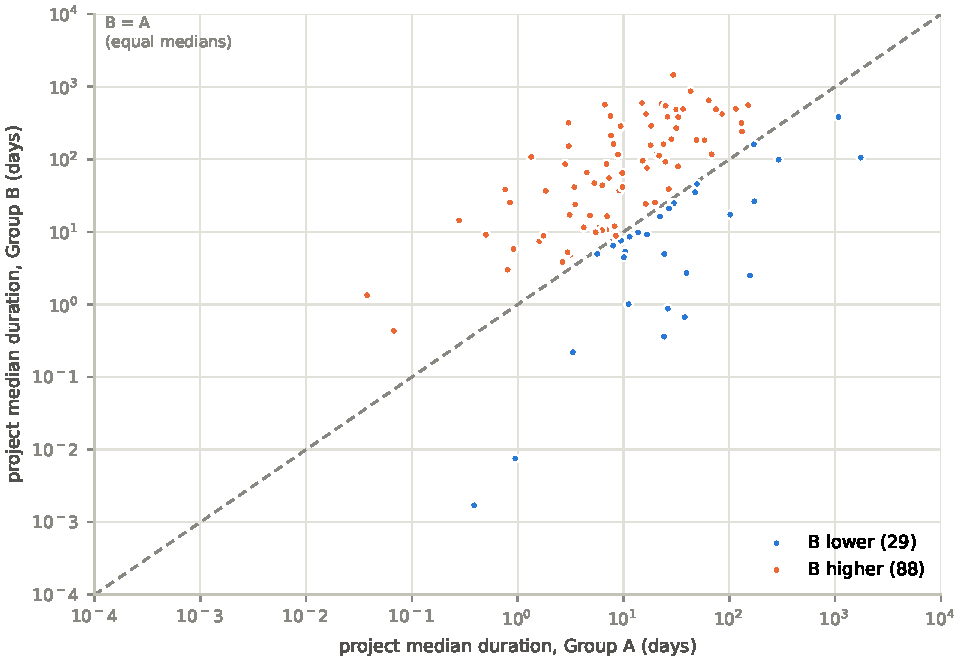
\includegraphics[width=.58\linewidth]{figures/fig4_projects.pdf}
\caption{Pairwise project comparison: median duration for single-PR ($x$) vs.\ multi-PR ($y$) issues across the \valnProjBoth{} projects containing both groups. Most projects lie above the equality line ($y=x$).\label{fig:projects}}
\end{figure}

A two-sided sign test across these \valnProjBoth{} projects reveals that multi-PR bugs have a higher median closure duration in \valnBhigher{} projects, while closing faster in only \valnBlower{} ($p=\valsignP$, median within-project difference \valmedProjDiff{}~days; Fig.~\ref{fig:projects}). Furthermore, a multivariate regression model predicting $\log(1 + \text{duration})$ with project fixed effects and creation-year fixed effects yields a highly significant Group-B coefficient ($\hat\beta = \valfeCoef$, 95\% CI \valfeCI{}, $p=\valfeP$), representing approximately a \valfePct\% increase in expected closure duration within the same repository and year. Table~\ref{tab:projects-top} summarizes the top 15 contributing projects; the complete list of all 117 projects is archived in the replication package.

\subsection{Dose-Response: Increasing PR Count}\label{sec:trend}
Treating the linked PR count $k$ as an ordinal metric, Spearman rank correlation between $k$ and closure duration is $\rho = \valrho$ ($p=\valrhoP$). As shown in Table~\ref{tab:categories} and Fig.~\ref{fig:category}, median duration increases from \valmedA{}~days at $k=1$, to 33.4~days at $k=2$, and 86.8~days at $k=3$. However, counts beyond $k=3$ represent rare outliers ($n=1$ for $k=4$, $n=2$ for $k \ge 5$); we caution against extrapolating trends into these sparse cells.

\begin{table}[t]
\centering
\caption{Median duration by number of matched linked PRs.\label{tab:categories}}
\small \begin{tabular}{@{}lrrr@{}}
\toprule
Linked PRs & $n$ & Median duration (d) & P90 (d) \\\midrule
1 & 14,280 & 8.0 & 280 \\
2 & 615 & 33.4 & 615 \\
3 & 44 & 86.8 & 878 \\
4 & 1 & 8.9 & 9 \\
5+ & 2 & 2,013.5 & 3,665 \\
\bottomrule
\end{tabular}
\par\vspace{2pt}{\footnotesize\textit{Note: categories 4 and 5+ contain $n\leq 2$ issues}}
\end{table}


\begin{figure}[htbp]\centering
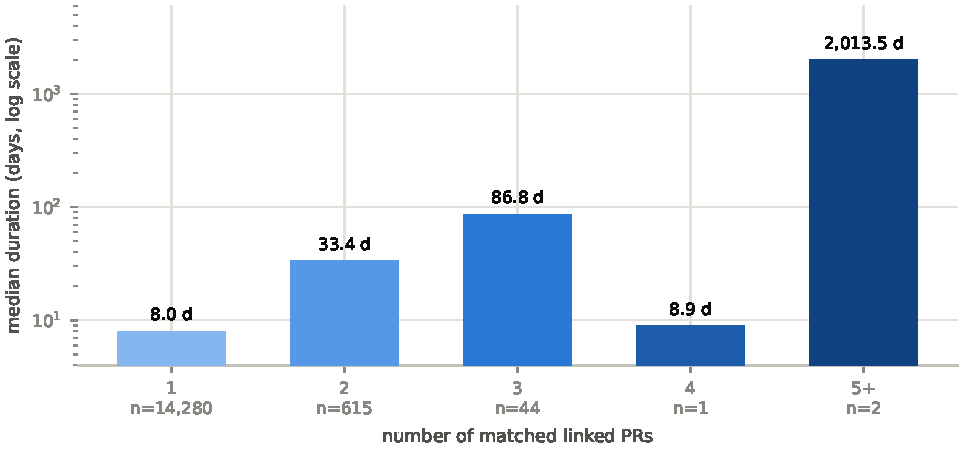
\includegraphics[width=.58\linewidth]{figures/fig3_kcategory.pdf}
\caption{Median closure duration categorized by linked PR count $k$, with sample counts annotated.\label{fig:category}}
\end{figure}

\subsection{Temporal Dynamics: When Do Linked PRs Arrive?}\label{sec:timing}
Evaluating the arrival timing of pull requests relative to issue lifespans provides critical insight into the underlying mechanism. Fig.~\ref{fig:timing} plots the relative creation time of each linked PR as a fraction of total issue lifetime ($0.0 = \text{creation}$, $1.0 = \text{closure}$).

\begin{figure}[htbp]\centering
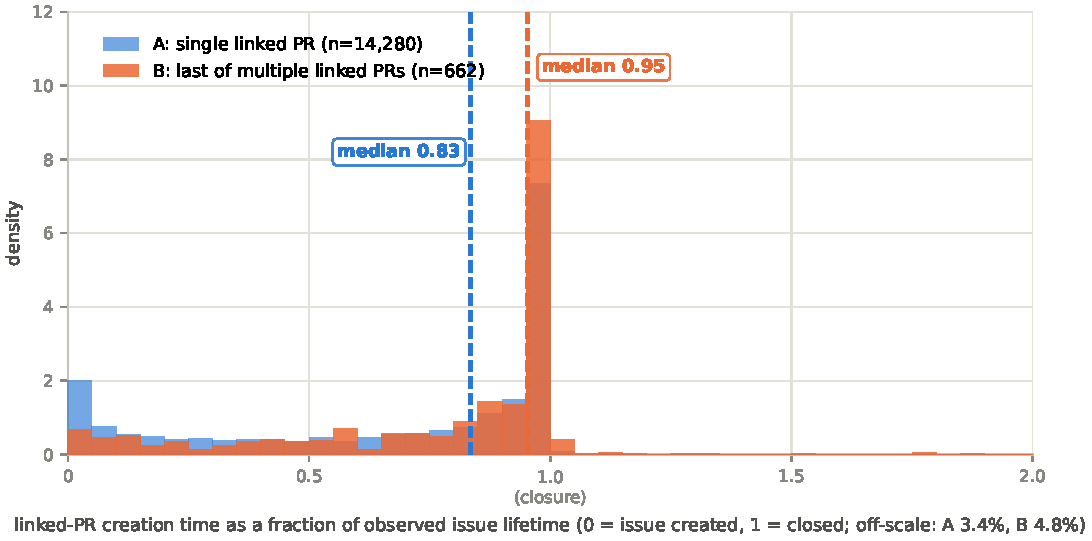
\includegraphics[width=.68\linewidth]{figures/fig5_timing.pdf}
\caption{Creation timing of linked pull requests as a fraction of issue lifespan ($0.0 = \text{opened}$, $1.0 = \text{closed}$). Dashed lines denote group medians.\label{fig:timing}}
\end{figure}

In Group A, the single resolving PR appears at a median of \valaFracMed\% of the issue's total lifespan. In Group B, the initial PR appears early (median \valtMedFirst\% of lifespan), but the \textbf{last linked PR arrives at a median of \valtMedLast\% of the issue's lifespan}. For \valtNinety\% of multi-PR issues, the final PR is submitted during the terminal 10\% of the issue's lifetime. This demonstrates that multi-PR issues are tickets where the PR link set continued to accumulate across the ticket's active open period—strongly pointing toward reverse causality and time accumulation.

\subsection{Label Classification Validation}\label{sec:validation}
Table~\ref{tab:validation} summarizes the validation audit of the strict-bug classification rule. Among the $\valvN$ randomly sampled cohort tickets, \valvConf{} were confirmed as genuine defects, \valvRej{} were rejected, and \valvUnc{} were classified as uncertain.

\begin{table}[t]
\centering
\caption{Label-validation audit of the strict-bug classification (seeded random sample of 100 cohort issues; LLM-assisted single-reviewer screening, not independent double-human validation).\label{tab:validation}}
\small \begin{tabular}{@{}lp{0.52\textwidth}@{}}
\toprule
Outcome & $n$ (of 100) \\\midrule
Confirmed as a genuine bug report & 91 \\
Rejected (not a bug report) & 2 \\
Uncertain & 7 \\
\midrule
Precision, decided cases only & \textbf{97.9\%} (95\% Wilson CI 92.5\%--99.4\%) \\
Precision, uncertain counted as errors & 91.0\% (CI 83.8\%--95.2\%) \\
\bottomrule
\end{tabular}
\end{table}


Among decided cases, strict-tier precision is \valvPrec{} (95\% Wilson score CI \valvCI). If every uncertain case is conservatively counted as misclassified, precision remains \valvPrecAll{} (95\% CI \valvCIAll). The two rejected tickets represented internal refactoring and CI infrastructure maintenance that had received automated bug labels. Uncertain tickets involved borderline subjective reports, such as gameplay difficulty tuning and ambiguous UX preferences. We reiterate that this audit evaluated precision via single-reviewer LLM-assisted screening; unlabelled defects omitted from the corpus cannot be detected via this protocol.
